\section{Results}

To simulate the inhibition of HDAC6-mediated uncoating by DARPin-F10 we created two new HDAC6 complex formation models: "Symmetric DARPin" and "Asymmetric DARPin" based, respectively on "Symmetric" and "Asymmetric" model variants, as reported in Chapter \ref{ch:ReactionModels}. The key difference between them follows from the structure of original models. Ub only assists the binding of myosin in "Asymmetric" model, so presence of DARPin-F10 would only inhibit myosin recruitment, while for "Symmetric" model DARPin-F10 would affect recruitment of both myosin and dynein motors.

\begin{figure}
\begin{center}
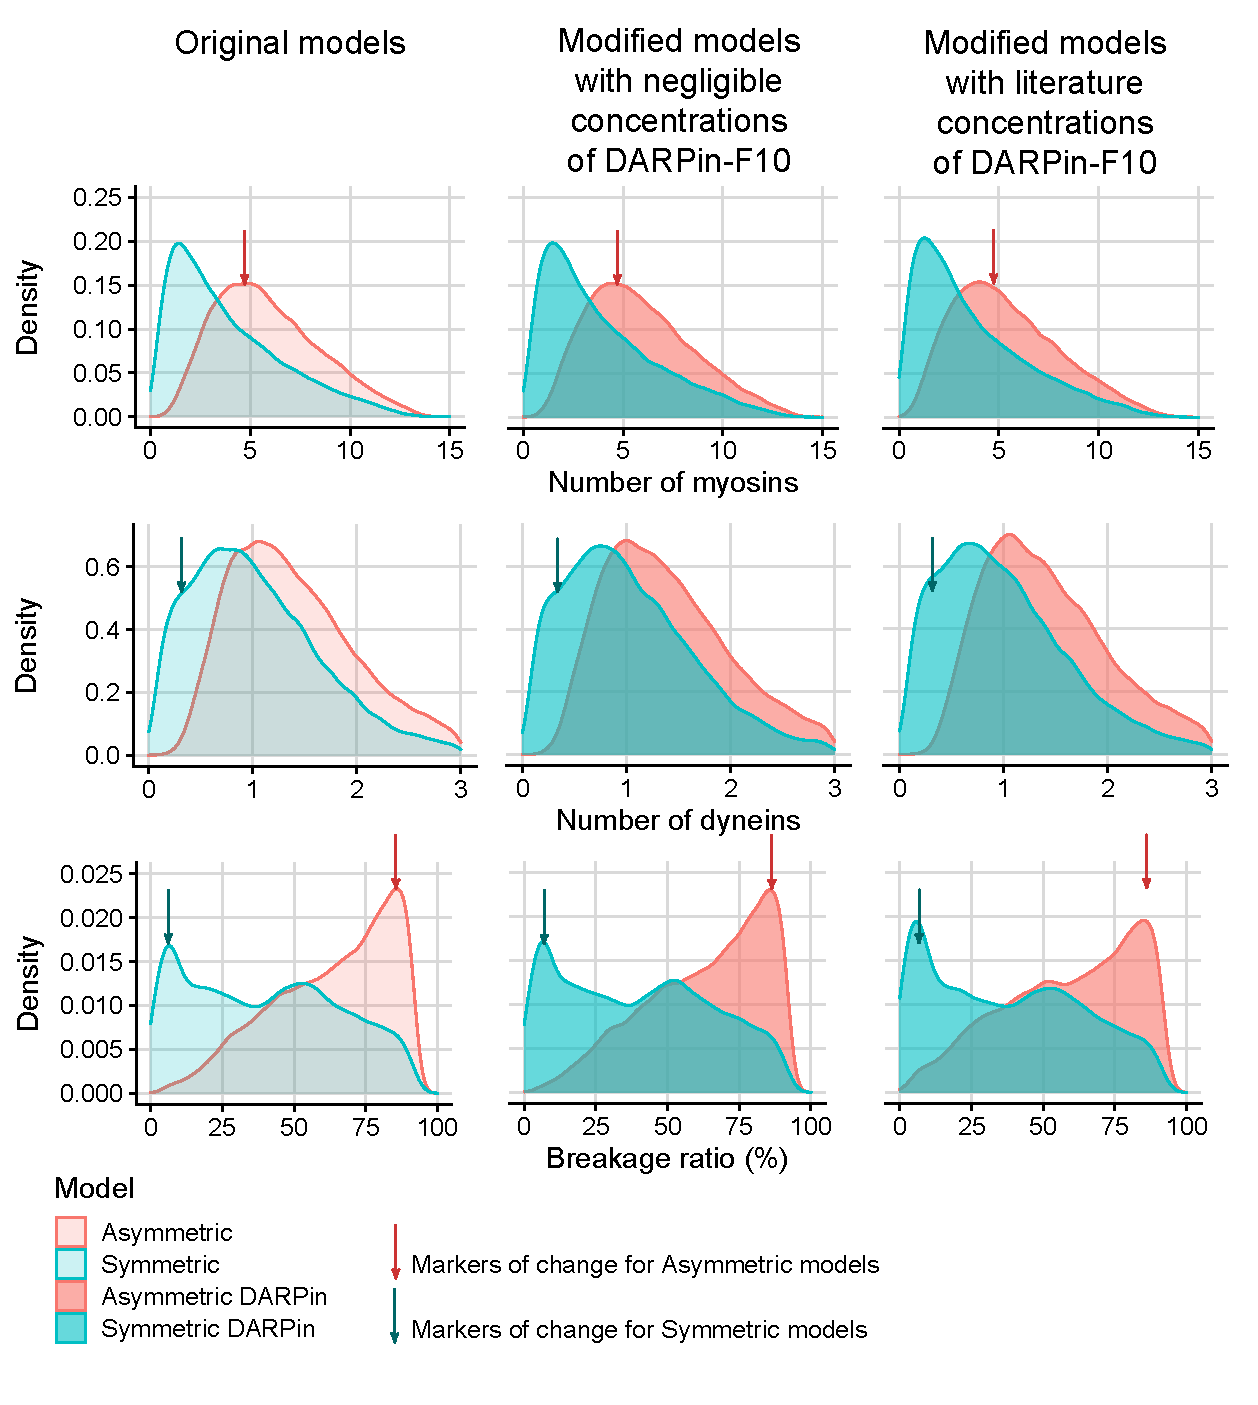
\includegraphics[width=0.95\textwidth, trim={0cm 0cm 0cm 0cm}, clip]{D_chapters/3_DARPinModels/Density_DARPin.pdf}
\caption[HDAC6 complex formation models densities with and without DARPin-F10]%
{HDAC6 complex formation models densities with and without DARPin-F10.}
\label{figure:darpinDensities}
\end{center}
\end{figure}

To verify that the base reaction network of our modified HDAC6 models functions as before, we uniformly sampled reactions and rates around our starting point for two concentrations of DARPin-F10 - one negligibly small, and another compatible with DARPin concentrations previously reported in literature (figure \ref{figure:darpinDensities}). Modified models with negligible concentrations of DARPin-F10 performed largely the same as before. While difference at literature reported concentrations wasn't striking, it is clear that modified Asymmetric DARPin model peak of myosin recruitment is shifted slightly towards 4 from 5 previously observed in original model. Likewise, modified Symmetric DARPin model on average recruits slightly fewer than dyneins than observed in the original. These changes in motor recruitment seem to lead to density increase in low capsid breakage ratio for Symmetric DARPin model and density decrease of high capsid breakage ratio for Asymmetric DARPin model (Figure \ref{figure:darpinDensities}).

\begin{figure}
\begin{center}
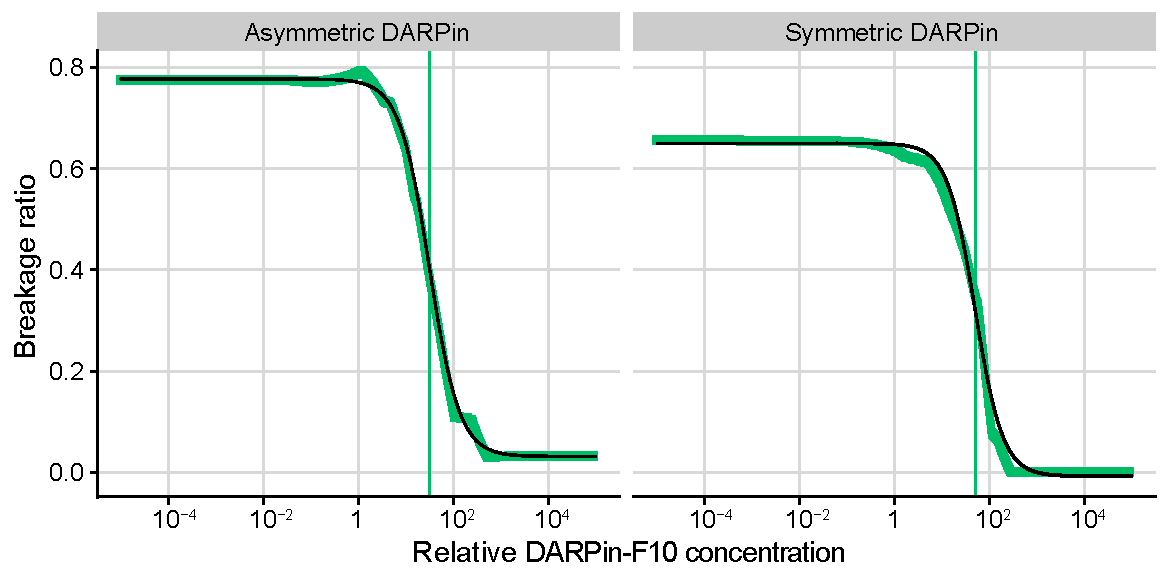
\includegraphics[width=0.95\textwidth, trim={0cm 0cm 0cm 0cm}, clip]{D_chapters/3_DARPinModels/FitDarpinTrajectories.pdf}
\caption[Capsid breakage prediction depending on relative DARPin-F10concentration]%
{Capsid breakage prediction depending on relative DARPin-F10 concentration. \par
Green trajectory is a direct prediction from the model, black line is a corresponding Hill equation fit. Vertical green line denotes EC50 value of the fit.}
\label{figure:darpinDensities}
\end{center}
\end{figure}

To simulate influenza uncoating dose response to DARPin-F10 we widely sampled DARPin-F10 concentration near literature value, and ran simulations for both "Symmetric DARPin" and "Asymmetric DARPin" models of HDAC6 complex formation. Both models displayed similar sigmoidal behavior. At low concentrations Breakage ratio for both models stayed approximately the same as before (Figure \ref{figure:sampledTrajectories}), with "Asymmetric DARPin" model variant achieving higher capsid breakage. Increasing DARPin F10 concentration lead to a dramatic drop in observed capsid breakage ratio.

To characterize resulting trajectories we fitted them using Hill equation for dose response. Notably, "Asymmetric DARPin" had lower half maximal effective concentration at approximately 1.1 $\mu$M, compared to "Symmetric DARPin" at approximately 1.7 $\mu$M.

To estimate effective DARPin-F10 concentrations, we used our Hill equation fits with estimates of DARPin-F10 efficiency we obtained from the experimental data provided by our collaborators \cite{DarpinData} (Table \ref{table:DARPinFittingCoefficients}). For the uncoating assays effective DARPin-F10 concentrations for both model variants ended up slightly under 1 $\mu$M. For viral growth curves they were approximately 2.5 $\mu$M for MOI = 0.05 PFU/ml, and 7 $\mu$M for MOI = 10 PFU/ml. These concentrations are significantly higher than our starting DARPin-F10 concentration of $34.7$ nM or cellular HDAC6 concentrations, but are not outside of bounds of reason for intracellular protein expression \cite{milo_2015}. As well as, \cite{guillard2017structural} uses biochemical assays with DARPin concentrations at 3 $\mu$M to characterise their binding kinetics.